%%**********************Partie 3 *********************** 


 \chapter{Mise en place d'un retour d'état et d'un pré-compensateur}
 \chaptermark{Retour d'état et pré-compensateur}

L'asservissement de position du système $S_{v_{m}\longmapsto v_{s}}$ , est réalisé selon la loi de commande par retour d'état :\\
 $v_{m}(t)=Nk_{e}\theta_{r}(t)-Kx(t)=Nv_{r}(t)-Kx(t)$ , avec : $K=[k_{1} \hspace{2mm} k_{2}]$.\\\\
 
 \section{Calcul des paramètre du retour d'état dans la base initial :}
 
\subsection{Détermination de l'expression du système ($A_{bf}$, $B_{bf}$, $C_{bf}$ et $D_{bf}$) :}

D'après notre système on a l'expression :\\
\\\\
$\dot{x}=Ax+Bv_{m}=Ax+B(Nv_{r}-Kx)=(A-BK)x+BNv_{r}$
\\\\
On obtient alors notre matrice dynamique \quad $A_{bf}$=(A-BK)\\
\\
et : \quad $B_{bf}$=B.N \\
 et :\quad $C_{bf}$=[1 0] \\
 et :\quad $D_{bf}$=[0] \\\\\\\\\\

\subsection{L'expression de $A_{bf}$ en fonction de $[k_{1}$,$k_{2}]$ : }

On a $A_{bf}$=(A-BK),  avec: $K=[k_{1} \hspace{2mm} k_{2}]$
D'ou :\\\\
$A_{bf}=
\begin{bmatrix} 
0 & \frac{K_{s}}{9K_{g}} \\
-\frac{K_{g}K_{m}}{T_{m}}.k_{2} & -\frac{K_{g}K_{m}}{T_{m}}.k_{2}-\frac{1}{T_{m}}
\end{bmatrix}$ \\\\

\subsection{Justification la possibilité de placer les V.P de la matrice $A_{bf}$ et calcul de K :}

On a les valeurs propres : $v_{1},v_{2}=-2.4\pm5.5j$ \\
et:\\
$A_{bf}=
\begin{bmatrix} 
0 & \frac{K_{s}}{9K_{g}} \\
-\frac{K_{g}K_{m}}{T_{m}}.k_{2} & -\frac{K_{g}K_{m}}{T_{m}}.k_{2}-\frac{1}{T_{m}}
\end{bmatrix}$ \\\\

L'expression du polynôme caractéristique est:\\
P($\lambda$)=$\lambda^2+(\frac{1}{T_{m}}-\frac{K_{g}K_{m}}{T_{m}}.k_{2})\lambda+\frac{K_{s}}{9K_{g}}.\frac{K_{g}K_{m}}{T_{m}}.k_{1}$\\\\

On place les valeurs propres à $p_{1},p_{2}=-2.4\pm5.5j$\\

On obtient alors le polynôme suivant: \\\\
$(\lambda+2.4+5.5j)(\lambda+2.4-5.5j)={\lambda}^2+4.8\lambda+36.01$\\\\

Et par identification avec le polynôme P($\lambda$) et en tenant compte des valeurs expérimentales de $K_{g} K_{m} K_{s}$ et$T_{m}$ , on trouve alors:  $k_1$=1.389à \quad $k_2$=0.5986 \hyperref[section1.1]{(voir Annexe)}\label{annexe1}\\



\section{Calcul des paramètres du retour d'état en utilisant la forme compagne de commande :}


\subsection{Loi de commande de la forme compagne de commande et L'expression du modèle du système asservi :  }

Dans cette partie, on a le système asservi par retour d'état nommé ($A_{cbf}$, $B_{cbf}$, $C_{cbf}$, $D_{cbf}$)\\ 

et le modèle d'espace d'état sous la forme compagne de commande est:\\\\

 $A_{cbf}=A_{c}-B_{c}k_{c}$.\\

 $B_{cbf}=B_{c}N$.\\

 $C_{cbf}=C_{c}$. \\
 
 et : \quad $D_{cbf}=0$.\\\\
 
 
\subsection{Expression de la matrice dynamique en fonction de $K_{1c}$ et $K_{2c}$ :}
 On pose $K_{c}=[k_{1c} \quad k_{2c}]$,\\ 

Et à partir de l'expression du polynôme caractéristique suivant : $ P(\lambda)=\lambda^2+\frac{1}{T_m}\lambda$, on a: \\\\

$A_{c}=\begin{bmatrix}
  0&1\\
  0&-\frac{1}{T_{m}}
    \end{bmatrix}$\\

\quad et : $B_{c}=\begin{bmatrix}

            0\\1
            \end{bmatrix}$ \\\\
et on remplace dans la forme de $A_{cbf}$ :\\ 
$A_{cbf}=A_{c}-B_{c}K_{c}$\\

$A_{cbf}=\begin{bmatrix}
0&1\\
0&-\frac{1}{T_{m}}
\end{bmatrix}
   - \begin{bmatrix}
     0\\1
   \end{bmatrix}. 
   \begin{bmatrix}
   k_{1c}&k_{2c}
   \end{bmatrix}$ \\\\
  
$\Longleftrightarrow \quad
A_{cbf}=\begin{bmatrix}
          0&1\\
          -k_{1c}&-\frac{1}{T_{m}}-k_{2c}
         \end{bmatrix}$\\\\
         
\subsection{Détermination de $K_{1c}$ et $K_{2c}$ :}

On veut obtenir des valeurs propres en boucle fermée : $v_{1},v_{2}=-2.4\pm5.5j$ \\         
         
On place dans l'expression du polynome :\\

$P(\lambda)={\lambda}^2+4.8\lambda+36.01$\\

et par identification des élements des matrices on a:\\
$\begin{bmatrix}
 0&1\\
 -k_{1c}&-\frac{1}{T_{m}}.k_{2c}
  \end{bmatrix}=\begin{bmatrix}
    0&1\\
   -36.01&-4.8
  \end{bmatrix}$\\\\
  avec : $T_{m}=0.3$\\

  
On obtient alors :\\
 $K_{1c}=36.01$ \quad
 et $K_{2c}=1.467$ \\\\

On a :$K=K_c.P^{-1}$ \\

Nous trouvons: $K=\begin{bmatrix}
               1.378&0.598
               \end{bmatrix}  $\\\\ 
                     
         
\subsection{Calcul de pre-compensateur N :}

Après l'ajout du gain $K$ par retour d'état,on remarque que les valeurs propres du la matrice sont égale aux valeurs propres qu'on souhait obtenir, alors le système est stable mais il existe un écart entre la consigne et la sortie $V_{s}$.\\
Et pour corriger cette erreur, on place un gain de pré-compensation sur l'entrée de la consigne.\\

et on calcule N permettant d'annuler l'erreur de position de l'asservissement($\varepsilon$=1), on a alors : N=$\frac{1}{C(A+BK)^{-1}.B.\varepsilon}$ \\

en tenant compte des valeurs expérimentales de $T_{m}$, $K_{m}$, $k_{1}$=0.6545 

on trouve: $N=k_{1}=0.655$\\

\subsection{Simulation du système asservi par retour d'état :}


\begin{center}
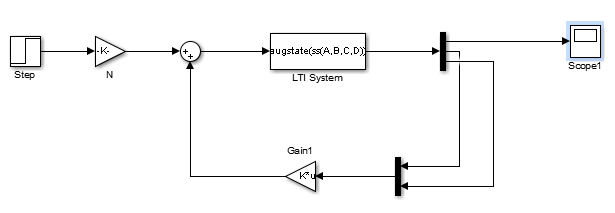
\includegraphics[scale=0.7]{simulink_retourdetat.PNG}
\captionof{figure}{\textit{asservissement par retour d'état.}}
\label{fig1} 
\end{center}











